
\section{Architecture Integration}

\subsection{Model Support}

\begin{table}[H]
\centering
\small
\begin{tabular}{llllll}
\toprule
\textbf{Architecture} & \textbf{Attention} & \textbf{RoPE?} & \textbf{GQA?} & \textbf{T5 bias?} & \textbf{Verified} \\
\midrule
DistilBERT & Flat & No & No & No &  \\
RoBERTa & Nested & No & No & No &  \\
GPT-2 & Causal & No & No & No &  \\
T5 & Causal + bias & No & No & Yes & {{T5\_VERIFIED}} \\
Qwen3.5 & Causal + RoPE & Yes & Yes & No & {{Q\_VERIFIED}} \\
\bottomrule
\end{tabular}
\end{table}

\subsection{Weight Transfer}

\subsubsection{DistilBERT (Flat)}

\begin{lstlisting}
q_lin: Linear(768, 768)
k_lin: Linear(768, 768)
v_lin: Linear(768, 768)
out_lin: Linear(768, 768)
\end{lstlisting}

Direct copy. \texttt{is\_nested\_encoder = False}.

\subsubsection{RoBERTa (Nested)}

\begin{lstlisting}
attention.self.query: Linear(768, 768)
attention.self.key: Linear(768, 768)
attention.self.value: Linear(768, 768)
attention.output.dense: Linear(768, 768)
\end{lstlisting}

Extract from inner \texttt{self}. The outer \texttt{attention.output.dense} is preserved 
via \texttt{IdentityOutProj} (identity, no operation).

\subsubsection{GPT-2 (Causal)}

\begin{lstlisting}
attn.c_attn: Conv1D(768, 2304)   # fused Q, K, V
attn.c_proj: Conv1D(768, 768)
\end{lstlisting}

Transpose \texttt{c\_attn} weight, split into Q/K/V.

\subsubsection{T5 (Relative Position Bias)}

T5 has \texttt{relative\_attention\_bias} embedding. We preserve it:

\begin{lstlisting}
if hasattr(src, "relative_attention_bias"):
    self.relative_attention_bias = src.relative_attention_bias
    self.has_relative_attention_bias = True
\end{lstlisting}

\subsection{Nested Encoder Handling}

For RoBERTa/BERT, we use \texttt{IdentityOutProj} for the inner attention's output 
projection:

\begin{lstlisting}
class IdentityOutProj(nn.Identity):
    lora_A = None
    lora_B = None
    def freeze_base_weights(self): pass
\end{lstlisting}

The outer \texttt{attention.output.dense} (in \texttt{BertAttention}) applies the actual 
projection.

\subsection{Causality}

For decoders, we apply the causal mask \textbf{before} the ramp:

\begin{lstlisting}
causal_tril = torch.tril(torch.ones((L, L), dtype=torch.bool))
scores = scores.masked_fill(~causal_tril, -10000.0)
# Then apply ramp on distances
\end{lstlisting}

For causal distance, $d_{ij} = \max(0, i - j)$.

\subsection{RoPE Handling}

RoPE is applied to Q, K \textbf{before} computing scores:

\begin{lstlisting}
Q, K = apply_rotary_pos_emb(Q, K, cos, sin, position_ids)
\end{lstlisting}

Then standard score computation, mask, ramp.

\subsection{Fast Path}

If all heads have \texttt{span + R >= L}, we skip ramp computation entirely. This 
avoids allocating $\mathcal{O}(H L^2)$ when unnecessary.

\begin{lstlisting}
span = torch.sigmoid(self.span_logits) * self.max_span
if not ((span + self.ramp_size) >= N_k).all():
    # allocate ramp
    ...
\end{lstlisting}

\subsection{Injection Algorithm}

\textbf{Algorithm 2:} Inject ASA-Span into a full model
\begin{lstlisting}
Input:  model M, config c, S_max, R
Output: M with ASA-Span attention

1:  for   in transformer_layers(M) do
2:      src $\leftarrow$ extract_attention( )
3:      if src is None: continue
4:      if is_already_adaptive_span(src): continue
5:      new $\leftarrow$ AdaptiveSpanAttention(config=c, pretrained_attn=src,
6:                                    max_span=S_max, ramp_size=R)
7:      replace_attention( , new)
8: end for
\end{lstlisting}

\subsection{Failure Handling}

\texttt{inject\_adaptive\_span} returns \texttt{None} on:
\begin{itemize}
\item Already-injected layer (AdaptiveSpan instance)
\item DeltaNet/LinearAttention layers (unsupported)
\item Weight extraction failure

\end{itemize}
\begin{lstlisting}
try:
    new_block = AdaptiveSpanAttention(...)
except Exception:
    return None
\end{lstlisting}

\subsection{Parameter Count}

\begin{table}[H]
\centering
\small
\begin{tabular}{ll}
\toprule
\textbf{Projection} & \textbf{Params} \\
\midrule
$W_Q$ & $d \cdot H d_h$ \\
$W_K$ & $d \cdot H_{kv} d_h$ \\
$W_V$ & $d \cdot H_{kv} d_h$ \\
$W_O$ & $H d_h \cdot d$ \\
Span logits & $H$ \\
\bottomrule
\end{tabular}
\end{table}

Total: same as MHA + $H$ extra parameters.

\subsection{Registry}

\begin{lstlisting}
@ATTENTION_REGISTRY.register("adaptive_span")
@ATTENTION_REGISTRY.register("adaptive_span_attention")
class AdaptiveSpanAttention(BaseAttention): ...
\end{lstlisting}

\subsection{Failure Modes}

\begin{lstlisting}

---
\end{lstlisting}

\begin{figure}[H]
\centering
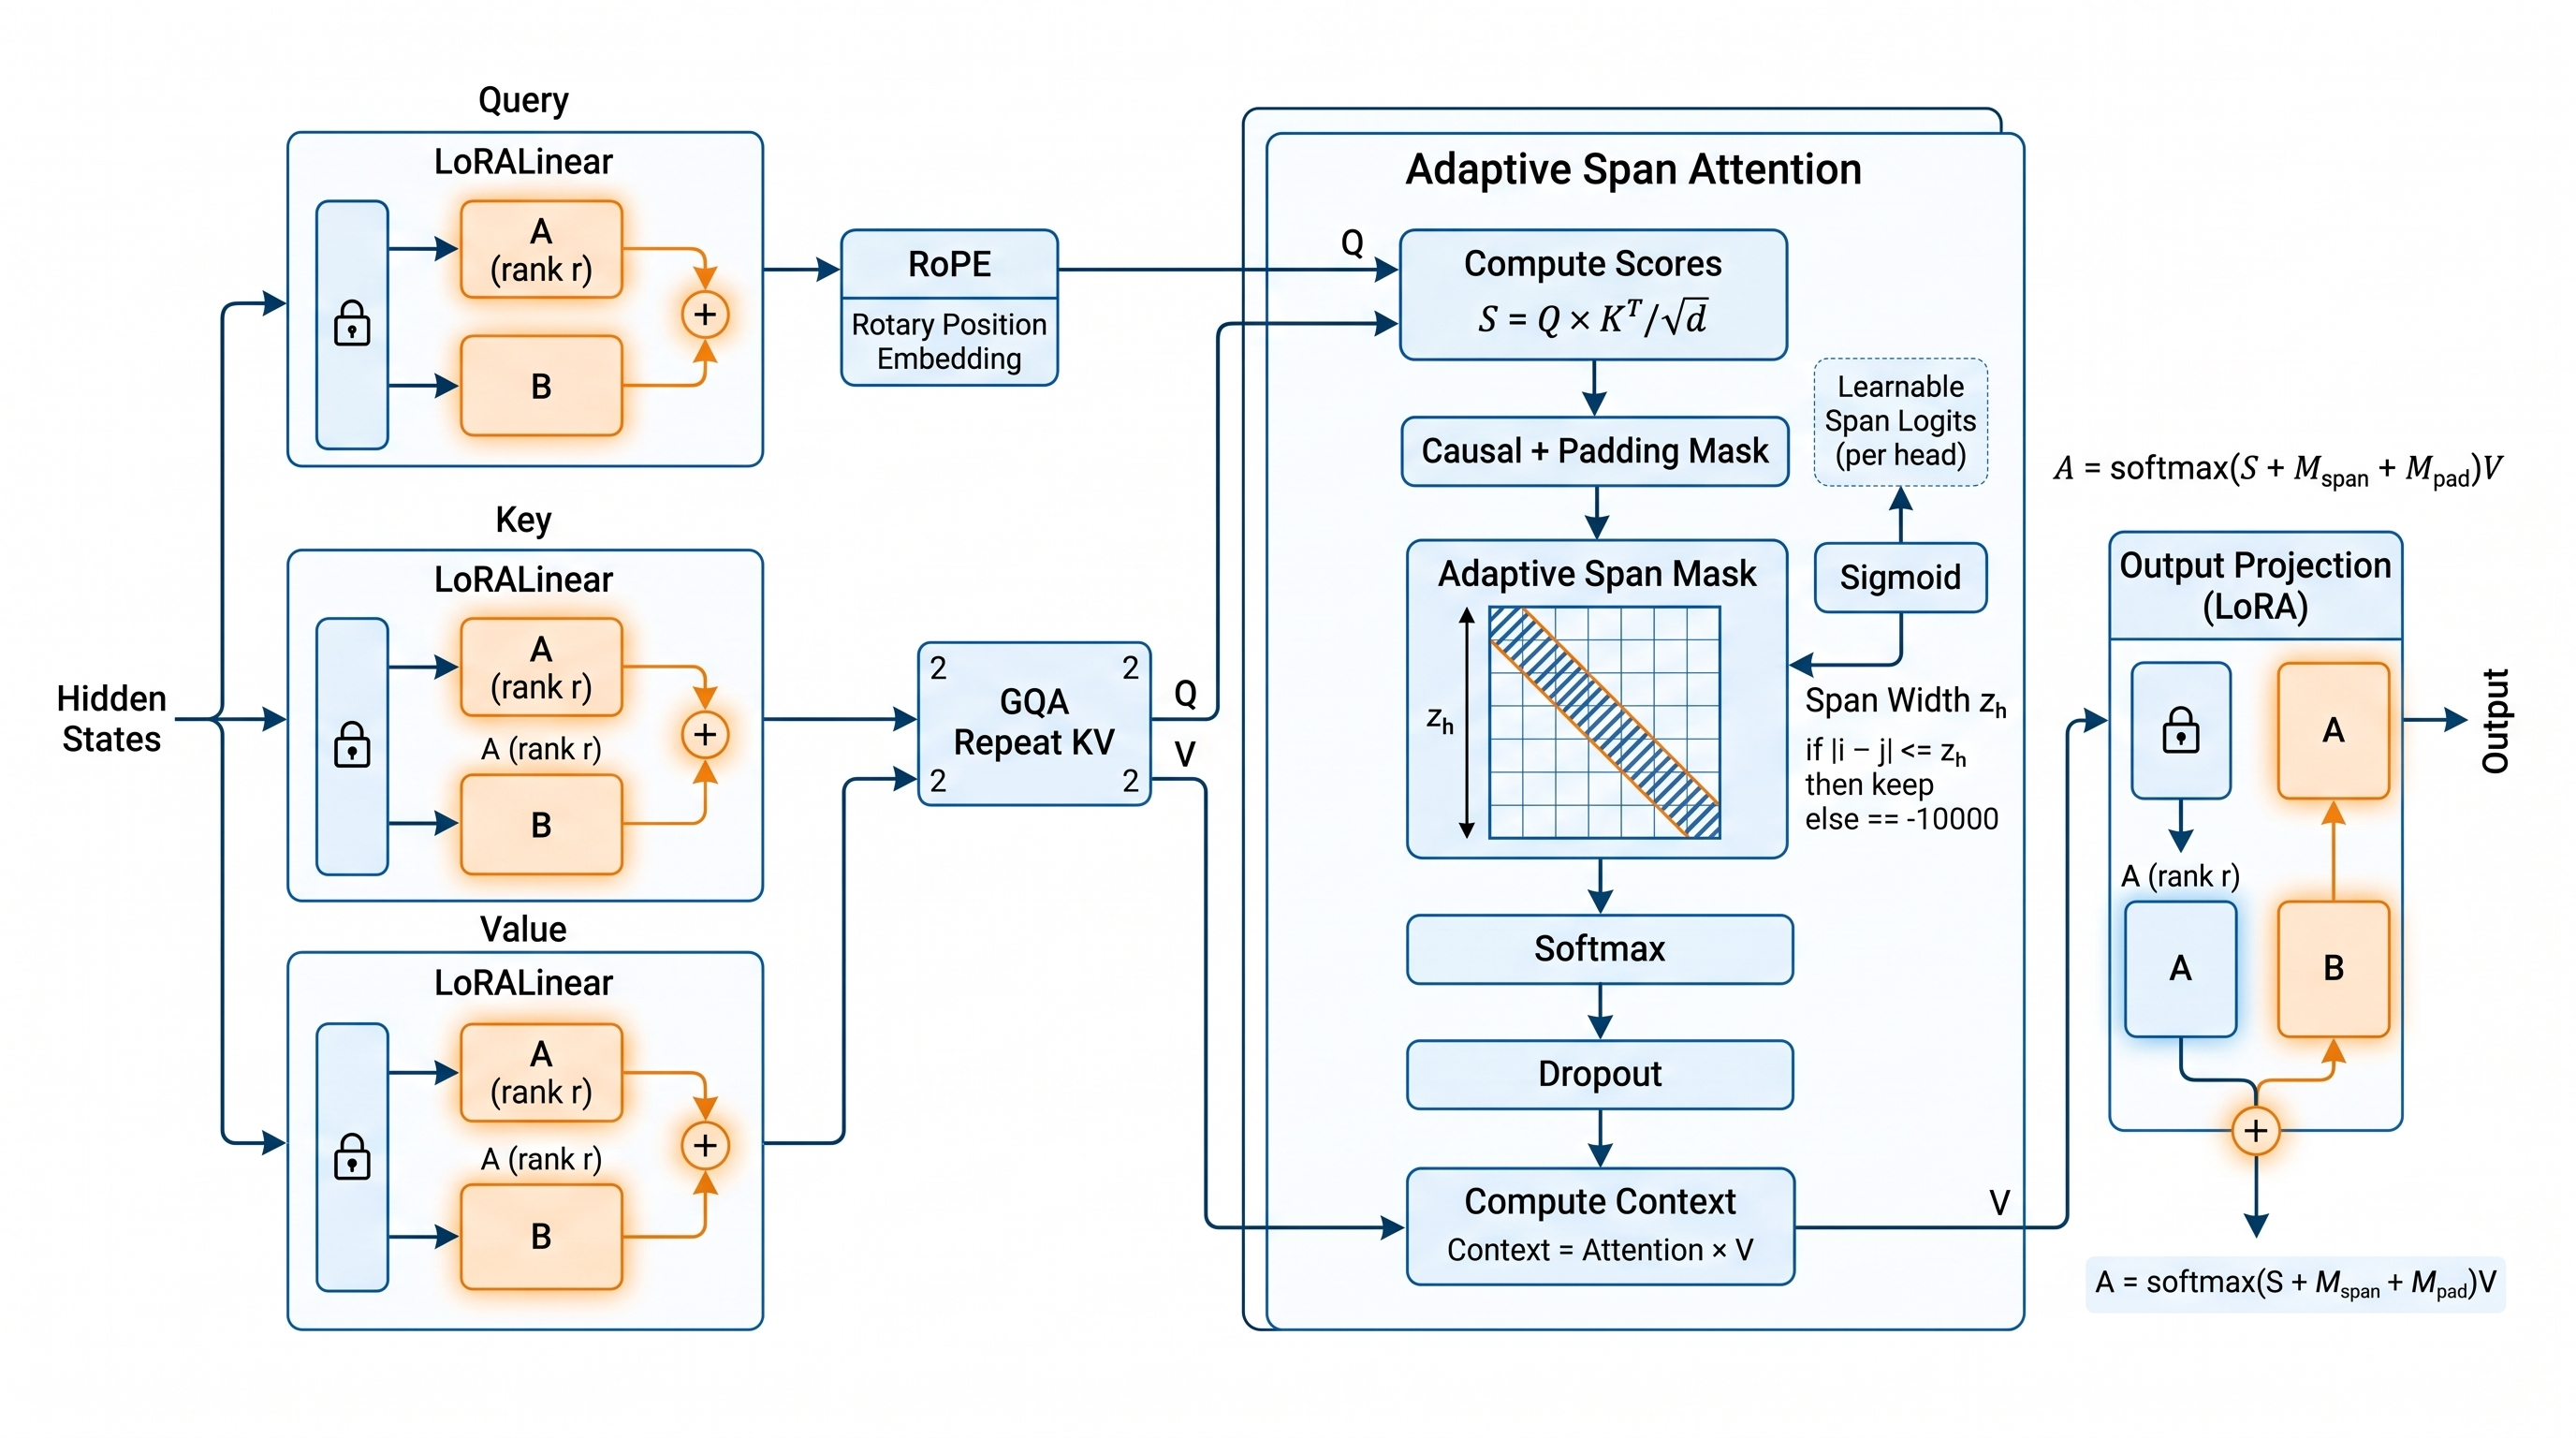
\includegraphics[width=\linewidth]{figures/architecture.jpeg}
\caption{High-level architectural diagram of AdaptiveSpanAttention.}
\label{fig:arch_AdaptiveSpanAttention}
\end{figure}

